\documentclass[11pt,a4paper]{article}
\usepackage[utf8]{inputenc}
\usepackage[T1]{fontenc}
\usepackage{graphicx}
\usepackage{hyperref}
\usepackage{listings}
\usepackage{caption}
\usepackage{tikz}
\usepackage{float}
\usetikzlibrary{positioning,arrows.meta}

\title{Practical Work 1: TCP File Transfer}
\author{Le Quy Ton}
\date{\today}

\lstset{
  basicstyle=\ttfamily\small,
  breaklines=true,
  frame=single
}

\begin{document}
\maketitle

\section*{1. Introduction}
This report documents an individual implementation of a one-to-one TCP
file transfer utility (client \& server) using POSIX sockets in C. The
purpose is to design a minimal protocol, implement the transfer over a
reliable TCP stream, and demonstrate end-to-end file delivery.

\section*{2. Protocol Design}
The protocol uses short ASCII headers exchanged before streaming raw binary
data. It is intentionally simple to avoid parsing complexity and to make
testing straightforward.

\subsection*{Protocol Steps}
\begin{enumerate}
  \item Client connects to server (TCP three-way handshake).
  \item Client sends header: \texttt{SEND <filename>\textbackslash n}.
  \item Server replies: \texttt{OK}.
  \item Client sends header: \texttt{SIZE <number>\textbackslash n}.
  \item Server replies: \texttt{OK}.
  \item Client streams raw binary file data (exactly \texttt{<number>} bytes).
  \item Server writes received bytes to disk under the received filename.
  \item Server replies: \texttt{DONE} and the connection may close.
\end{enumerate}

\clearpage
\section*{3. Protocol Diagram}

\begin{figure}[htbp]
  \centering
  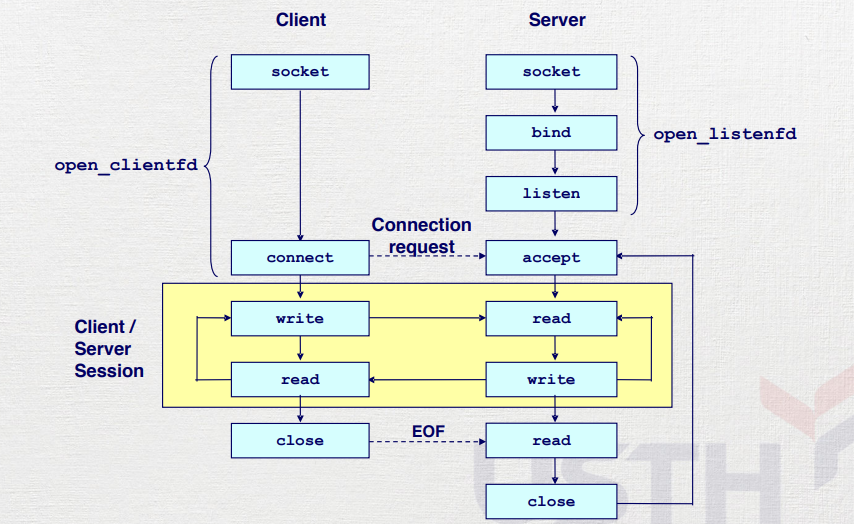
\includegraphics[width=0.92\textwidth]{diagram.png}
  \caption{Socket-level workflow: open, connect/accept, write/read, close.}
  \label{fig:protocol_image}
\end{figure}

\section*{4. System Organization}
\begin{itemize}
  \item \textbf{Client:} Establishes TCP connection (socket(), connect()),
    sends metadata headers and streams file bytes (send()).
  \item \textbf{Server:} Listens on a port (socket(), bind(), listen()),
    accepts connection (accept()), reads headers, receives bytes (recv())
    and writes them to disk.
\end{itemize}

\section*{5. Implementation}
Below is a concise description of how the transfer is implemented and a
short illustrative snippet showing the exchange of headers (not the full
program).

\subsection*{Runtime sequence}
\begin{enumerate}
  \item Server: create socket, setsockopt(SO\_REUSEADDR), bind(port), listen().
  \item Client: create socket, connect(server\_ip, port).
  \item Client sends 'SEND <filename>\textbackslash n'; server reads and responds 'OK'.
  \item Client sends 'SIZE <numBytes>\textbackslash n'; server responds 'OK'.
  \item Client: read file in chunks and \texttt{send()} them to server.
  \item Server: loop \texttt{recv()} until total bytes received == <numBytes>, write chunks to file.
  \item Server sends 'DONE' and either closes or waits for next connection (design choice).
\end{enumerate}

\subsection*{Minimal code snippet illustrating header exchange}
\begin{lstlisting}[language=C, basicstyle=\ttfamily\footnotesize]
/* client side (concept) */
sprintf(buf,"SEND %s\n", filename);
send(sock, buf, strlen(buf), 0);
recv(sock, buf, sizeof(buf), 0); /* expect "OK" */

sprintf(buf,"SIZE %d\n", filesize);
send(sock, buf, strlen(buf), 0);
recv(sock, buf, sizeof(buf), 0); /* expect "OK" */

/* then stream binary bytes via send() */
\end{lstlisting}

\subsection*{Notes on robustness}
\begin{itemize}
  \item All \texttt{recv()} return values must be checked (0 = peer closed,
    negative = error).  
  \item Use a loop to accumulate partial reads/writes until the declared
    file size is reached.  
  \item Consider basic sanity checks: file size limit, filename validity,
    and handling abrupt disconnects.
\end{itemize}
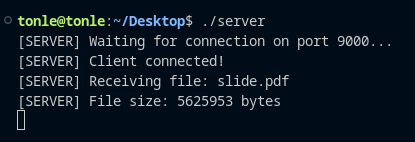
\includegraphics[width=0.5\textwidth]{server.png}
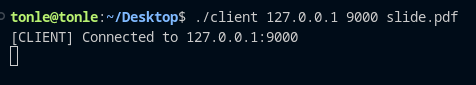
\includegraphics[width=0.5\textwidth]{client.png}
\section*{7. Work distribution}
This practical work was completed individually by the author. All design,
implementation and testing steps were done by myself.

\section*{8. Conclusion}
A minimal TCP-based file-transfer protocol was designed and implemented.
The system demonstrates reliable file delivery over TCP using a small,
clear protocol and can be extended for multiple clients, authentication,
or reliability checks if required.

\end{document}
